% This Document is Copyright 2018 the authors.

% Misc. notes:
% - On model comparison figure: stuff <-60 deg more affected by gaia scan pattern, mass-loss history and stellar pop variation, disk contamination

\documentclass[twocolumn]{aastex62}

\addtolength{\topmargin}{-0.25in}
\addtolength{\textheight}{0.50in}
\setlength{\parindent}{\baselineskip}

\newcommand{\acronym}[1]{{\small{#1}}}
\newcommand{\package}[1]{\textsl{#1}}
\newcommand{\Gaia}{\textsl{Gaia}}
\newcommand{\gaia}{\textsl{Gaia}}
\newcommand{\hst}{\textsl{HST}}
\newcommand{\articlename}{\textsl{Letter}}
\newcommand{\sectionname}{Section}
\newcommand{\lcdm}{\acronym{$\Lambda$CDM}}
% \newcommand{\Tycho}{\textsl{Tycho}}
% \newcommand{\DRone}{\textsl{\acronym{DR1}}}
\newcommand{\DRtwo}{\textsl{\acronym{DR2}}}
% \newcommand{\TGAS}{\textsl{\acronym{TGAS}}}
% \newcommand{\DPAC}{{\acronym{DPAC}}}
% \newcommand{\documentname}{\textsl{Note}}
% \newcommand{\equationname}{equation}

% \newcommand{\AU}{\mathrm{A.U.}}
% \newcommand{\dd}{\mathrm{d}}
% \newcommand{\given}{\,|\,}
% \newcommand{\T}{^{\mathsf{T}}}
% \newcommand{\inv}{^{-1}}
\newcommand{\kpc}{\textrm{kpc}}
\newcommand{\msun}{\textrm{M}_\odot}

\shorttitle{dynamical evidence of a dark halo substructure}
\shortauthors{bonaca et al.}

\begin{document}\sloppy\sloppypar\raggedbottom\frenchspacing

\title{\textbf{%
Encounter of the GD-1 stellar stream with a massive perturber:\\
Dynamical evidence of a dark substructure in the Milky Way halo
}}

\correspondingauthor{Ana Bonaca}
\email{ana.bonaca@cfa.harvard.edu}

\author[0000-0002-7846-9787]{Ana Bonaca}
\affil{Harvard--Smithsonian Center for Astrophysics, 60 Garden St, Cambridge, MA 02138, USA}

\author[0000-0003-2866-9403]{David W. Hogg}
\affil{Center for Cosmology and Particle Physics, Department of Physics, New York University, 726~Broadway, New York, NY 10003, USA}
\affil{Center for Data Science, New York University, 60 Fifth Ave, New York, NY 10011, USA}
\affil{Max-Planck-Institut f\"ur Astronomie, K\"onigstuhl 17, D-69117 Heidelberg}
\affil{Flatiron Institute, 162 Fifth Ave, New York, NY 10010, USA}

\author[0000-0003-0872-7098]{Adrian~M.~Price-Whelan}
\affil{Department of Astrophysical Sciences, Princeton University, Princeton, NJ 08544, USA}

\author[0000-0002-1590-8551]{Charlie Conroy}
\affil{Harvard--Smithsonian Center for Astrophysics, 60 Garden St, Cambridge, MA 02138, USA}

\begin{abstract}\noindent
% The GD-1 stellar stream is a long, thin, cold stream of stars in the Milky Way halo.
% It is sensitive to details of halo dynamics, and it has been shown to have structure that is suggestive of non-trivial gravitational interactions in its past.
We present a conceptual model for the interaction of the GD-1 stellar stream with a massive perturber that---without fine-tuning---explains many of the features of one of the stream structures, including a gap and an off-stream spur of stars.
The model involves an impulse by a fast encounter, after which the stream grows a loop of stars on different orbital energies which, at specific viewing angles, appears off the stream track.
% The model involves an impulse by a fast encounter, after which the stream grows a loop of stars that is both off the stream track, and on a set of orbits with different frequencies.
The configuration-space observations are sensitive to a the mass, age, impact parameter, and total velocity of the encounter, and future velocity-space observations will be sensitive to the full velocity vector of the perturber.
Quantitative comparison of the spur and gap features prefers models where the perturber is in the mass range $10^6\,\rm M_\odot$ to $10^8\,\rm M_\odot$.
% Given sensible assumptions about age and velocity, the perturber must have had a mass in the range $10^6\,\rm M_\odot$ to $10^8\,\rm M_\odot$.
Orbit integrations back in time show that the stream encounter could not have been caused by any known globular cluster or dwarf galaxy, and mass, size and impact-parameter arguments show that it could not have been caused by a molecular cloud in the Milky Way disk.
The most plausible explanation for the gap-and-spur structure is an encounter with a dark matter substructure, like those which are naturally predicted in this mass range in this part of the Milky Way halo in \lcdm\ cosmology.
% - leave possibility of a black hole
This observation opens up the possibility that detailed observations of streams could measure the mass spectrum of dark-matter substructures and even identify individual substructures and their orbits in the halo.

% We present a conceptual model for the interaction of GD-1, a thin Milky Way stellar stream, with a massive perturber.
% Following the encounter, the stream develops a gap at the location of the closest approach, from which emanates a loop of stream stars.
% Projected on the sky, this loop appears to extend from the stream as a narrow spur, thus reproducing the observed GD-1 morphology.
% Under the impulse approximation, we infer the length scale of impact (?) $GMT/BV = x$ from relative sizes of the gap and spur in GD-1(?).
% Encounters of GD-1 with known satellites and the Galactic disk have $GMT/BV \ll x$.
% Given how GD-1 orbits far from the Galaxy (or some better argument here), the most plausible perturber is a dark matter subhalo, which naturally populate galactic halos in the $\Lambda$CDM cosmology.
% Future kinematic maps of the perturbed region of the GD-1 stream will put constraints on the mass spectrum of dark matter subhalos in the Milky Way.

\end{abstract}

\keywords{%
cosmology:~observations
  ---
dark~matter
  ---
gravitation
  ---
stars:~kinematics~and~dynamics
  ---
Galaxy:~halo
  ---
Galaxy:~kinematics~and~dynamics
}

\section{Introduction}
\label{sec:intro}
In the currently preferred \lcdm\ cosmological model of cold dark matter (CDM) with dark energy ($\Lambda$), dark matter forms clumps of arbitrarily low masses \citep[e.g.,][]{springel2008}.
Through mergers, these clumps grow to become massive halos that consist of a number of lower mass clumps, or subhalos \citep[e.g.,][]{whiterees1978}. 
Baryons can only be retained in halos more massive than $\sim10^8-10^9\,\rm M_\odot$ \citep[e.g.,][]{efstathiou1992, bullock2000}, which agrees well with the lowest-mass galaxies discovered around the Milky Way \citep[e.g.,][]{sg2007, martin2008}.
A critical prediction of CDM paradigm is the existence of dark subhalos less massive than $\lesssim10^8\,\rm M_\odot$.

Alternative cosmological models have been proposed that behave like \lcdm\ on large scales, but have no structure on small scales.
In the case of warm dark matter \citep[e.g.,][]{bode2001}, this is accomplished with a dark matter particle that is less massive ($m\sim\rm\, keV$) than the cold dark matter particle ($m\gtrsim10\rm\, GeV$), and thus streams out of the lowest mass clumps.
The fuzzy dark matter model \citep[e.g.,][]{hu2000} posits an ultra-light dark matter particle ($m\sim10^{-22}\rm\, eV$) that exhibits quantum behavior on macroscopic scales, which prevents collapse of halos less massive than $\sim10^7\,\rm M_\odot$.
Therefore, a ruling on the existence of low-mass dark matter subhalos would place strong constraints on the nature of dark matter \citep[e.g.,][]{bullockmbk2017, buckleypeter2017}.

Albeit dark, low-mass subhalos should still exert gravitational influence, so a number of searches for dark matter structure on small scales have been launched.
In a cosmological setting, gravitational lensing is our most sensitive method of detecting gravitational perturbations.
And indeed, some strongly lensed galaxies require the presence of a subhalo in the lens plane to fully explain the distribution of light in the lensed system.
To date, subhalos in the mass regime $10^8-10^9\,\rm M_\odot$ have been identified in a number of lenses \citep[e.g.,][]{vegetti2012,hezaveh2016}.
However, these objects are expected to host stars (although at luminosities below the current detection threshold), so the search for lower mass, and truly dark, subhalos continues, primarily by increasing the sample size of analyzed lenses.

In the local universe, dynamically cold stellar streams are promising devices for measuring detailed properties of the matter distribution \citep[e.g.,][]{johnston1999, bh2018}.
Formed by stars escaping a disrupting globular cluster at slightly offset orbital energies, stellar streams are one-dimensional structures in the 6D phase space.
An encounter between a stellar stream and a dark matter subhalo would perturb the orderly structure of the stellar stream, produce a gap in the stream density \citep[e.g.,][]{carlberg2012}, and, depending on the impact geometry, possibly also fold a part of the stream \citep[e.g.,][]{yoon2011}.
More than 40 thin stellar streams have been discovered in the Milky Way halo \citep{gc2016}, and the most prominent ones have already been searched for evidence of density variations.
The abundance of dark matter subhalos down to $\sim10^6\,\rm M_\odot$ inferred from the number and sizes of detected gaps is consistent with the \lcdm\ predictions \citep[e.g.,][]{carlberg2012,cg2013}.
In addition to dark matter subhalos, a number of physical processes can perturb streams at this level \citep[e.g.,][]{kupper2008, amorisco2016}.
As a result, no stream has definitively established the presence of dark matter substructure.

So far, studies of stream gaps have been statistical in nature, mainly because the data were not good enough to identify individual gaps at high confidence.
However, thanks to the recently released \gaia\ data \citep{gdr2}, identification of stream member stars has become extremely efficient \citep[e.g.,][]{malhan2018}.
In turn, this has enabled the discovery of a perturbation site in the GD-1 stream \citep{pwb} -- a prime candidate for dark matter influence on a stellar stream.

In this work, we follow up this initial discovery with the first in-depth analysis of a perturbed stellar stream.
We first review the observed properties of GD-1 (\S\,\ref{sec:data}), and then develop a fiducial model of a perturbed stream that qualitatively matches GD-1 observations (\S\,\ref{sec:model}).
Next, we explore the range of impact parameters allowed by the spatial distribution of GD-1 (\S\,\ref{sec:perturber_properties}), and make predictions for its kinematics (\S\,\ref{sec:kinematics}).
Finally, we discuss the limitations of the current modeling framework (\S\,\ref{sec:caveats}), possible origin of the perturber (\S\,\ref{sec:origin}), and suggest strategies to distinguish between different origin scenarios (\S\,\ref{sec:future}).


% The clustering of dark matter (DM) on scales smaller than dwarf galaxies remains one of the most pressing unknowns in cosmology and galaxy formation \citep[for a recent review, see][]{Bullock:2017}. % TODO: also Buckley summary?
% Dark matter theories predict different minimum mass scales for clustering: In the \lcdm\ model, DM subhalos with negligible baryonic content are expected to exist in abundance with arbitrarily low masses \citep{Green:2004, Springel:2008}, while alternative models (e.g., warm DM, self-interacting DM, axion DM) have larger cut-off masses in the DM power spectrum that depend on the parameters of these models \citep{Bode:2001, Spergel:2000, Peebles:2000, Mocz:2017}.
% The detection of dark but massive substructure would therefore place strong constraints on the physics of dark matter \citep[e.g.,][]{Buckley:2017}.
% 
% Two promising prospects for detecting such structures are (1) through microlensing within and between images of strongly-lensed galaxies \citep{Vegetti:2012}, and (2) using thin stellar streams around the Milky Way \citep{Johnston:2002, Ibata:2002}.
% Thin stellar streams form from the disruption of low-mass stellar systems like globular clusters and dwarf galaxies \citep{TODO} and are thus dynamically cold structures that form through phase-mixing of tidal debris over many orbits around the Galaxy.
% Cold but dynamically old streams stretch into long, thin streams of stars that are extremely sensitive to gravitational perturbations: a gravitational encounter between a dark massive substructure and a stream leaves imprints of the encounter in the form of irregular morphological features (loops, spurs, and folds) and density variations along the stream \citep{SiegalGaskins:2008, Carlberg:2009, Yoon:2011, Ngan:2016}.
% The density variations typically evolve to form spatial under-densities --- typically referred to as ``gaps'' --- that encode information about the perturber structure, perturber orbit, and time of encounter \citep{Yoon:2011, Carlberg:2012, Carlberg:2013, Erkal:2015, Erkal:2015b}.
% 
% For low-mass perturbers ($M \lesssim 10^7~\msun$), the characteristic scale of density variations is small, $\delta\rho / \rho \sim XX\%$, and therefore requires low-contamination selection of stream stars to detect.
% For this reason, not all stellar streams within the Milky Way are equally useful for studying the presence of dark substructure: some streams lie in regions of high background density where measuring small density variations is limited by Poisson variations of the background (e.g., Hermus/Hyllus; \citealt{Grillmair:2014}), some streams cross close to the Galactic center and disk where the Galactic bar and/or molecular clouds can leave density features (e.g., Ophiuchus and Palomar 5; \citealt{Price-Whelan:2016, Pearson:2017, Amorisco:2016}), and the densest known streams are often dynamically young and very cold, so epicyclic density variations naturally arise from the formation of the stream (e.g., the Palomar 5 stream; \citealt{Kupper:2008, Kupper:2015}).
% 
% The GD-1 stream \citep{Grillmair:2006, Price-Whelan:2018} is one of the most prominent stellar streams in the Milky Way halo and has many characteristics that make it an ideal place to study the small-scale density variations that would arise from gravitational interactions with dark matter substructures.
% The stream was discovered using a matched-filter on photometry from the Sloan Digital Sky Survey (SDSS; \citealt{SDSS, TODO}).
% GD-1 is relatively close to the Sun ($d_\odot \sim 8$--$12~\textrm{kpc}$), spans at least $100^\circ$ on the sky, and is at high Galactic latitude ($20^\circ \lesssim b \lesssim 60^\circ$) where Galactic background contamination is less significant.
% Already with its discovery, hints of density variations were apparent in the surface density and map of the stream (e.g., \figurename~XX in \citealt{Grillmair:2006}).
% However, with only photometric data, the background density at the limiting magnitude of the SDSS was too high to strongly conclude about the density structure of GD-1.
% 
% Subsequent work used Megacam to obtain deeper imaging across $\approx 45^\circ$ of GD-1 (APW: check this number).
% Using a matched-filter (here with the 2-band photometry from Megacam), it became clear that the density structure of GD-1 contains prominent under-densities (gaps) and ``wiggles'' in the mean track of the stream \citep{deBoer:2018}.
% These features again suggested the tantalizing possibility that GD-1 has encountered a massive perturber.
% 
% Previous work on the GD-1 stream relied primarily on filtering photometric data to map the stream.
% Recently, using astrometric data from the second data release (\DRtwo) of the \gaia\ mission \citep{TODO}, we combined a photometric matched-filter with a kinematic matched filter to select a high-purity sample of main-sequence stars in the GD-1 stream \citep{Price-Whelan:2018}.
% The velocity of GD-1 is distinct from the foreground Galactic disk stars over most of its extent, and is much colder than the stellar halo, so the combined selection provided the highest-contrast view of a thin stellar stream in the Milky Way to date.
% With this low-contamination selection of the stream, we (1) extended the footprint of the stream to $\approx 100^\circ$, (2) confirmed the existence of at least two prominent under-densities, and (3) identified two morphological features offset from the main track of the stream (the spur and blob).
% These non-trivial features of the stream are not expected from standard models of stream formation, and therefore further motivate studying their formation.
% 
% In this \articlename, we explore the interpretation that density variations and morphological anomalies along the GD-1 stream are a result of a gravitational interaction with a dark, massive perturber.
% In \sectionname~\ref{sec:model}, we ...


% \section{Encounter of GD-1 with a massive perturber}
% \section{Methods}
\section{Observed features of the GD-1 stellar stream}
\label{sec:data}
GD-1 is the longest ($>100^\circ$, 10\,kpc) thin ($\sigma\approx12'$, 30\,pc) stellar stream discovered in the Galactic halo \citep{gd2006}.
Based on its width and length, GD-1 is expected to be extremely informative about the global distribution of matter in the Galaxy \citep{lux2013, bh2018}.
Indeed, dynamical modeling of GD-1 individually, and in concert with the tidal tails of the Palomar~5 globular cluster, has already revealed that the inner dark matter halo is spherical \citep{koposov2010, bowden2015, bovy2016}.
Furthermore, \citet{cg2013} used data from the Sloan Digital Sky Survey \citep[SDSS,][]{york2000} to identify gaps in stellar density along GD-1 and concluded that the number, size and depth of GD-1 gaps is consistent with $\Lambda$CDM predictions of stream perturbation by dark-matter subhalos.
However, density variations in streams at the SDSS depth can originate in part from variations in the distribution of field Milky Way stars \citep{ibata2016}, so an increase in signal-to-noise is required to ascertain the true density structure of GD-1.

\begin{figure*}
\begin{center}
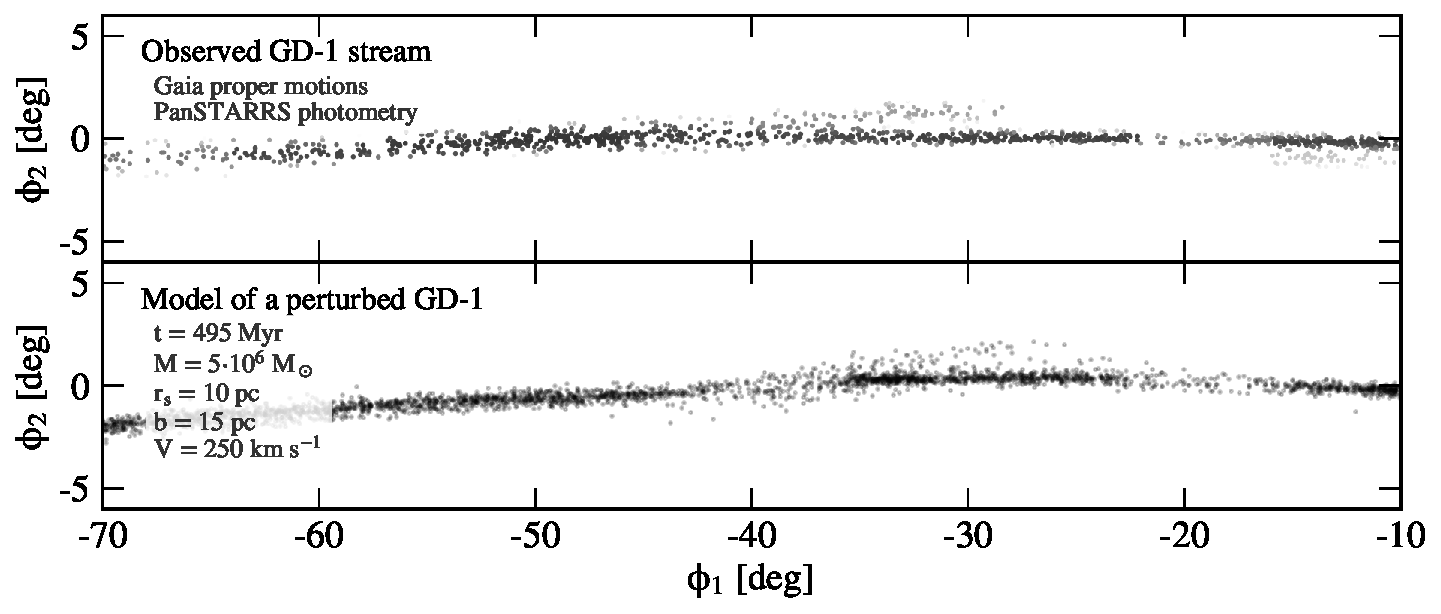
\includegraphics[width=0.9\textwidth]{../plots/stream_encounter.png}
\end{center}
\caption{Likely members of the GD-1 stellar stream, cleanly selected using Gaia proper motions and PanSTARRS photometry, reveal an underdensity in the stream and a spur extending for $\approx10^\circ$ from this gap (top).
% The gap is $\approx8^\circ$ wide and is located at $\phi_1\approx-40^\circ$ (top right).
An idealized model of GD-1 that has been perturbed by a compact, massive object (bottom).
The orbital structure of stars closest to the passing perturber is distorted into a loop of stars that after 0.5\,Gyr appears as an underdensity coinciding with the observed gap, and extends out of the stream similar to the observed spur.
% edge-on and matches the extent of the observed spur, as well as the location and the width of the gap.
}
\label{fig:fiducial}
\end{figure*}

Recently, \citet{pwb} used proper motions from the \gaia\ mission \citep{gdr2} and photometry from PanSTARRS \citep{ps} to confidently separate GD-1 stars from the Milky Way field stars.
This contamination-free view of GD-1 enabled the first unambiguous detection of gaps in a stellar stream, which remain evident in deeper imaging \citep{deboer2018}.
Additionally, the combined astrometric and photometric selection reveals GD-1 stars offset from the main stream track: an extended spur at $(\phi_1, \phi_2)\approx(-33^\circ,1^\circ)$ and a diffuse blob at $(\phi_1, \phi_2)\approx(-14^\circ,-1^\circ)$ in GD-1 coordinates.
Patterns imparted by the complex selection function, confusion by background galaxies, or foreground dust do not coincide with these GD-1 features; instead, they are inherent properties of the stream itself.

To highlight the complex structure of the GD-1 stream, we present the distribution of likely stream members at the top of Figure~\ref{fig:fiducial}.
As a first step in finding likely members, we followed \citet{pwb} in selecting stars consistent with an old and metal-poor population at a distance of 8\,kpc, and moving retrograde with respect to the Galactic disk, with proper motions in the GD-1 reference frame $(\mu_{\phi_1}, \mu_{\phi_2})\approx(-7,0)\;\rm mas\,yr^{-1}$.
The spatial distribution of these stars in the $\phi_2$ direction (i.e. perpendicular to the stream) is modeled as a combination of a constant background, a stream component at the location of the main stream track, and one additional Gaussian components on either side of the main stream to capture stream features beyond the main track.
We solved for the normalization, position and width of every component by exploring the parameter space with an ensemble MCMC sampler \citep{Foreman-Mackey:2013}.
We used 256 walkers that ran for a total of 1280 steps, and kept the final 256 steps to generate posterior samples in these parameters.
The above procedure is a full-stream generalization of the calculation in \citep{pwb} that quantified the fraction of stars in the additional components at the locations of the spur and the blob.
Finally, we define stream membership probability, $p_{mem}$, as the joint probability of a star belonging either to the main stream or the additional feature, and evaluate these probabilities using MCMC samples for every star.
Figure~\ref{fig:fiducial} shows stars with $p_{mem}>0.5$, with larger and darker points representing stars with a higher membership probability.

Most likely GD-1 members trace a thin stream, whose width varies between $\sigma\approx'$ and $'$.
% $\sigma\approx'$ at $\phi_1\approx-13^\circ$ to $\sigma\approx'$ at $\phi_1\approx-50^\circ$.
Stellar density along the stream is not uniform, with the most significant underdensities, or gaps, located at $\phi_1\approx-40^\circ$ and $\phi_1\approx-20^\circ$.
Additional components are above the background density in the spur region, $\phi_1\approx-35^\circ$, and the blob region, $\phi_1\approx-15^\circ$, and consistent with zero along the rest of the stream.
In the following section we present a conceptual model of GD-1 that simultaneously explains the gap in the stream and the spur extending from the stream.

\section{Modeling the perturbed GD-1 stream}
\subsection{Setup and the fiducial model}
\label{sec:model}
Unlike the observed GD-1, a globular cluster disrupting on the GD-1 orbit in a simple --- analytic and smooth --- galaxy creates a stream that is also smooth \citep{pwb}.
This model follows stars as they leave the progenitor, and accounts for their epicylic motion relative to the progenitor's orbit \citep{kupper2008, kupper2010, fardal2015}.
The resulting pattern of over- and underdensities is much more uniform than the observed stream, so the full extent of density variations in GD-1 cannot be simply explained by the process of globular cluster disruption alone.
As inhomogeneities can also be introduced into a stellar stream by adding a perturbation to the gravitational potential \citep[e.g.,][]{sgv2008}, in this Section we present a model of the GD-1 stream that had a recent, close encounter with a dense, massive object.

As a first step in creating a model of the GD-1 stream, we follow \citet{pwb} in finding the orbit of the GD-1 progenitor by fitting the six-dimensional phase-space distribution of GD-1 stars.
We assume a spherical logarithmic potential with a circular velocity of 225\,km\,s$^{-1}$ for orbit integration.
This simple gravitational potential is very close to the best-fit model of GD-1 \citep{koposov2010, bowden2015}, and it also allows much faster force evaluations than the standard, multi-component model of the Milky Way.
We then assume that the GD-1 progenitor was a globular cluster of initial mass $7\times10^4\rm\,M_\odot$ and half-light radius \,pc.
In our model, it started losing stars through evaporation 3\,Gyr ago and completely disrupted 300\,Myr before the present day.
We follow the progenitor's dissolution by releasing test particles from its Lagrange points, and produce a streakline model of the stream \citep{fardal2015}.
Although idealized, such models capture detailed properties of the more realistic, N-body, simulations of disrupting globular clusters \citep{kupper2012}.
The present day distribution of test particles is shown in GD-1 coordinates in the bottom of Figure~\ref{fig:fiducial}.
Had the progenitor survived to the present, it would be located at $\phi_1=-20^\circ$.
Instead, this model has a gap at that location, which coincides with the gap observed in GD-1.
The progenitor's initial mass and time of disruption were chosen to reproduce the stream width and the morphology of the more depleted observed gap.

To produce the second gap, our model also includes a massive and dense object on an orbit that crosses GD-1.
The object is represented by a \citet{hernquist1990} sphere of mass $5\times10^6\rm\,M_\odot$ and scale radius 10\,pc.
Its closest approach to GD-1 happened 495\,Myr with a relative distance of 15\,pc, which is smaller than the stream width.
The perturber came closest to GD-1 stars that are presently at $\phi_1\approx-38^\circ$.
During the encounter, nearby stars received a velocity kick from the perturber, and started moving towards the location of its closest approach.
In case of a weaker perturbation, e.g., one produced by a more diffuse perturber, the most significant component of the velocity kick is along the stream, which changes the orbital period of affected stars \citep{eb2015}.
On one side of the perturber, the affected stars have shorter orbital periods and hence speed by the unaffected stars, while on the other side they take longer to orbit the Galaxy, and lag behind the unaffected stream stars.
This creates a gap at the projected location of the closest approach, with a pile-up of stars on either side of the gap creating a signature double-horned profile \citep{carlberg2012}.
However, the perturber in our model is dense, so it imparts a significant velocity kick perpendicular to the stream as well as along the stream.
This leads to a loop of stars straying beyond the unperturbed stream track.
At the present, this loop is viewed edge-on and looks like the observed spur (Figure~\ref{fig:fiducial}, bottom).

% \subsection{Fiducial model}
The stream model in the bottom of Figure~\ref{fig:fiducial} qualitatively matches many features in the observed GD-1 stream (Figure~\ref{fig:fiducial}, top).
Not only are both of the most prominent gaps reproduced at the right location and with the right size, but their density contrast is matched as well.
The gap at $\phi_1\approx-20^\circ$, modeled as a disrupted progenitor, is almost completely depleted, while the gap at $\phi_1\approx-40^\circ$, the location of the impact, still retains some stars.
Furthermore, the model features a spur of the correct offset from the main stream and correct length.
It is not a perfect model, for example, the model stream extends past the observed extent of GD-1.
Still, this model is a remarkably realistic rendition of the observed GD-1, so we next quantitatively explore the range of impact parameters that produce a good match to the observed stream.

% \section{Results}
\subsection{Properties of the GD-1 perturber}
\label{sec:perturber_properties}
In our fiducial model of the GD-1 stellar stream (Section~\ref{sec:model}), the encounter with a perturber introduced a gap in the stream and ejected a spur of GD-1 stars beyond the main stream.
In this section, we constrain the range in perturber's mass and size, its impact parameter, velocity, and time of perturbation that reproduce well the location and width of the gap, and the location and extent of the spur.

\begin{figure*}
\begin{center}
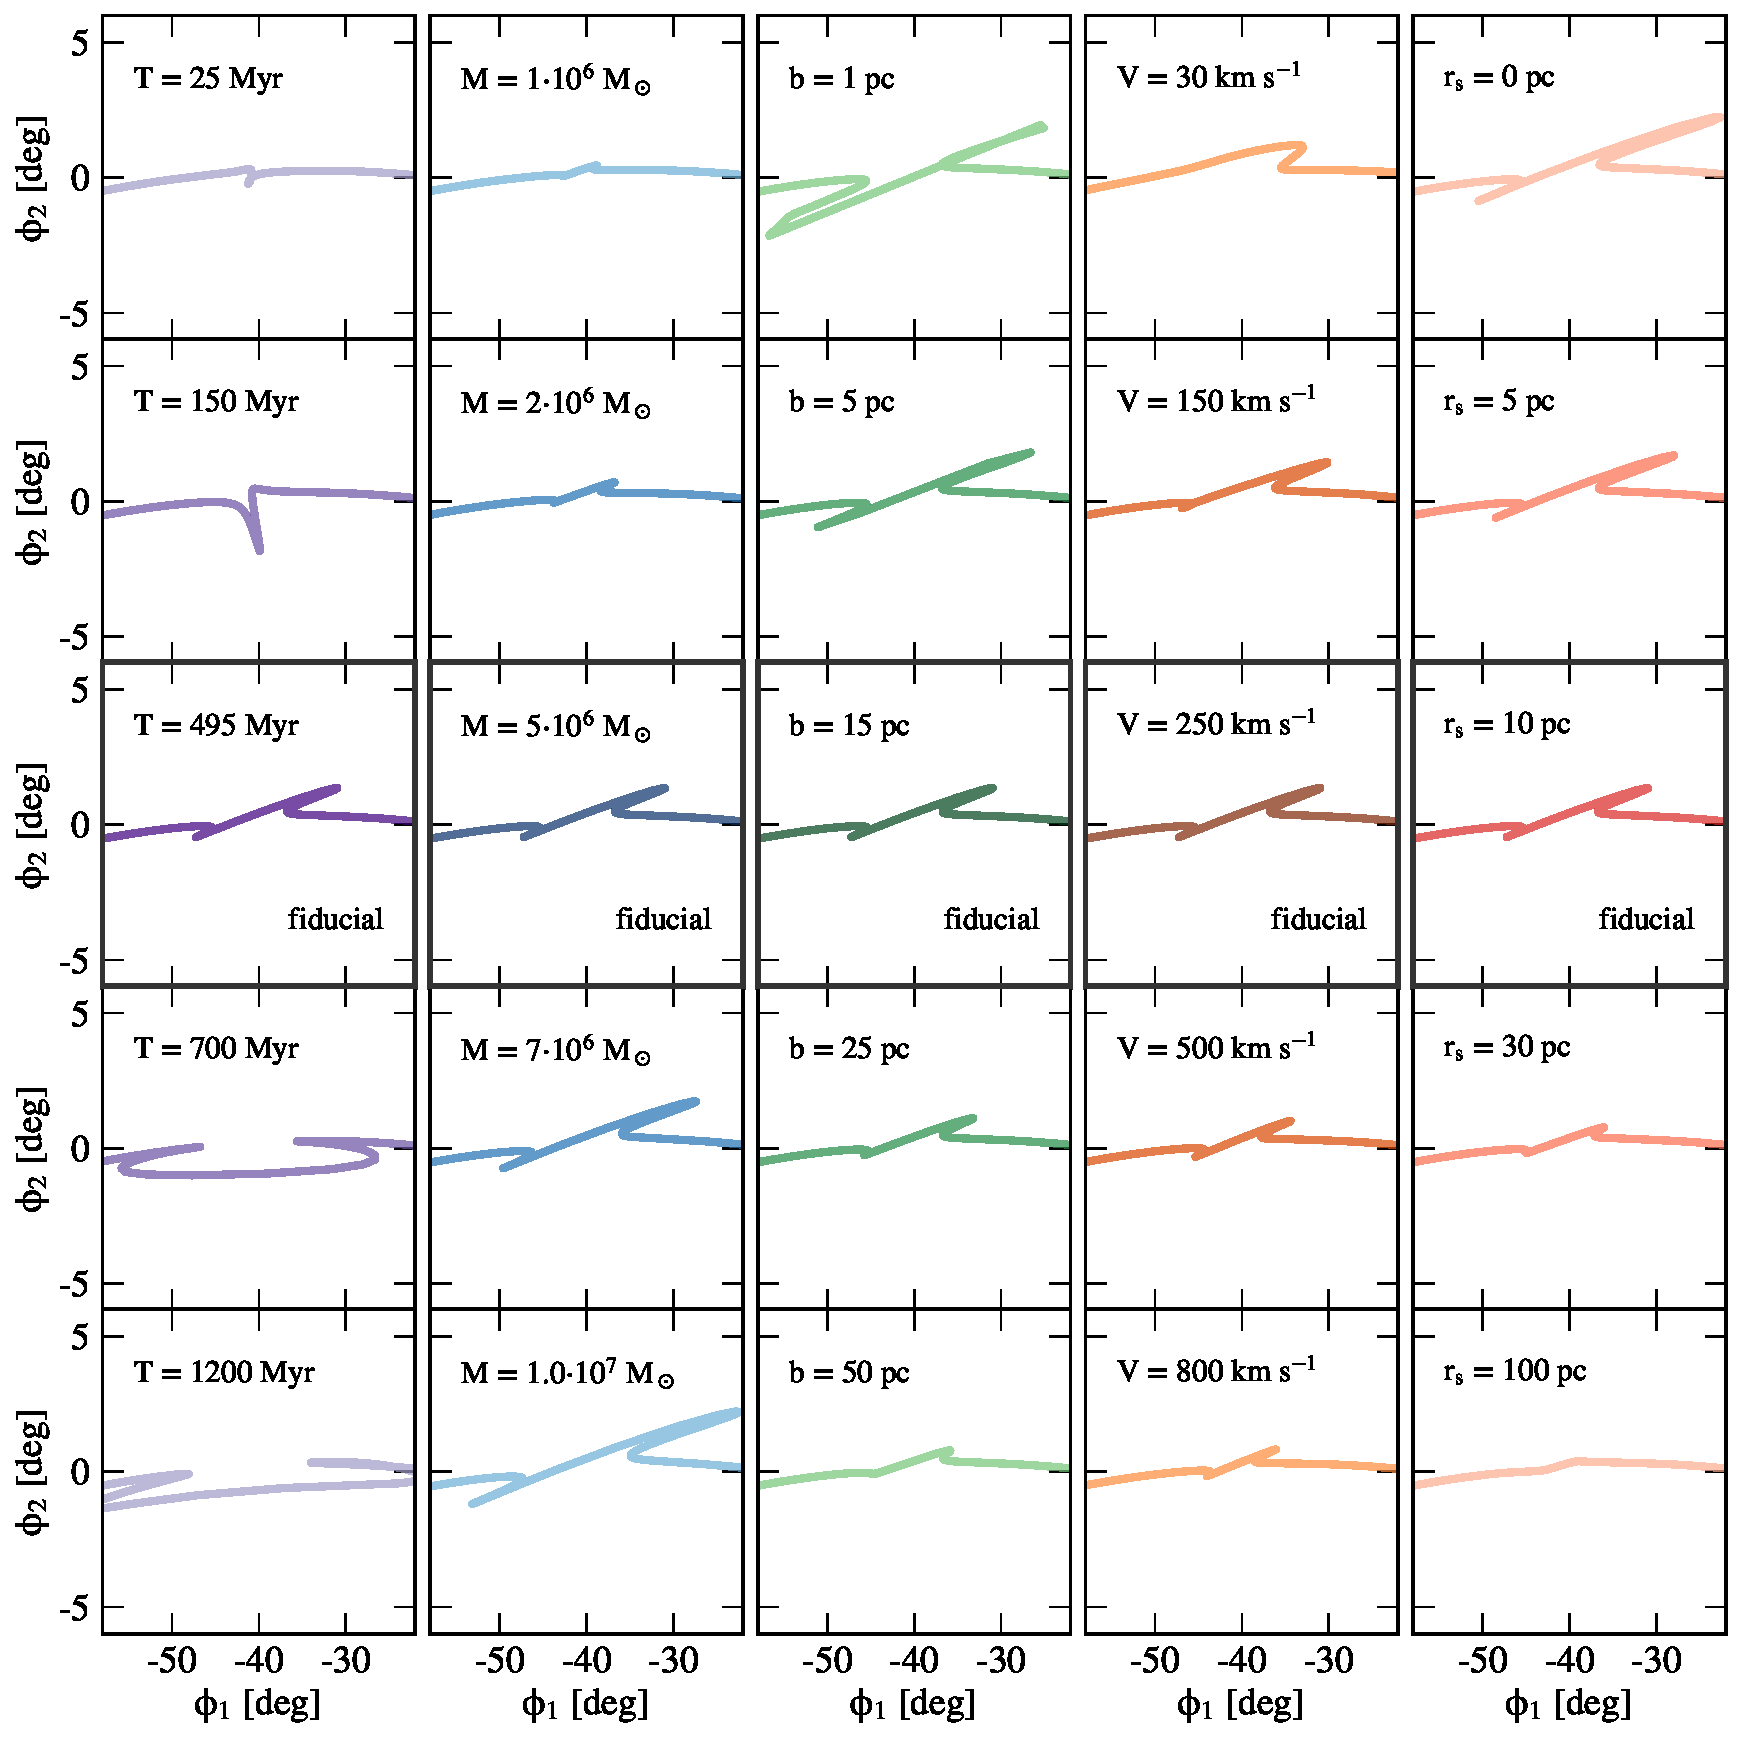
\includegraphics[width=0.9\textwidth]{excursions.pdf}
\end{center}
\caption{The stream response to different encounter parameters in columns from left: the time of impact, perturber's mass, its impact parameter, velocity and size.
The value of the varied parameter (given in the top left of every panel) increases from top to bottom, while all the other parameters are at their fiducial values (given in the middle row).
Signatures of perturbation become more prominent with an increase in time after the impact and mass of the perturber, and with a decrease of its impact parameter, velocity and size.
The relative sizes of the gap and the loop, and the loop orientation, break some of these degeneracies.
}
\label{fig:scalings}
\end{figure*}

To efficiently explore the allowed parameter space, in this section we assume that GD-1 stream stars share the orbit with their progenitor.
This allows for even faster generation of a stream model, at the expense of less realistic density contrasts along the stream.
In the third row of Figure~\ref{fig:scalings} we show our fiducial model of perturbed GD-1 under this assumption.
The perturber parameters have the same normalization as a model presented in the previous section.
However, since the stream is misaligned from the orbit \citep{sb2013}, the orientation angles between the GD-1 and perturber's orbit are different in the two cases.
This model also features a loop of stars removed from their original orbit, which projects to the GD-1 spur location at $\phi_1\gtrsim-40^\circ$, opens a gap at $\phi_1\approx-40^\circ$ and reconnects to the leading tail at $\phi_1\lesssim-40^\circ$.

With a method at hand to quickly generate stream models that reproduce basic features observed in GD-1, we explore how the stream morphology depends on impactor's properties.
We consider five parameters: time of impact, $T$, perturber's mass, $M$, its impact parameter, $b$, velocity, $V$, and size, $r_s$.
Each column of Figure~\ref{fig:scalings} shows models where one of the parameters is changed, while the others are kept at their fiducial values.
Parameter values are increasing from top to bottom (as labeled in top left of every panel), with the fiducial values shown in the middle row.
Most of the presented models preserve the angle between the loop and the unperturbed stream, while the main differences are in the width of the gap and the extent of the loop.

As the mass of the perturber increases, imparted velocity kicks to stream stars are larger, and the resulting loop and gap also increase in size.
The effects of other parameters are similar, for example, increasing the perturber's size (making it less dense) decreases the loop and gap sizes.
Indeed, bottom right panel of Figure~\ref{fig:scalings} shows a model perturbed with an object following the $\Lambda$CDM concentration--mass relation \citep{diemer2018}, and it shows no signature of a loop.
Given time, both the loop and the gap grow in size.
However, older loops are more aligned with the stream (Figure~\ref{fig:scalings}, bottom left panel), and hence more difficult to detect observationally.
The presence of a spur alone already implies that GD-1 had a recent encounter with a dense perturber.

\begin{figure*}
\begin{center}
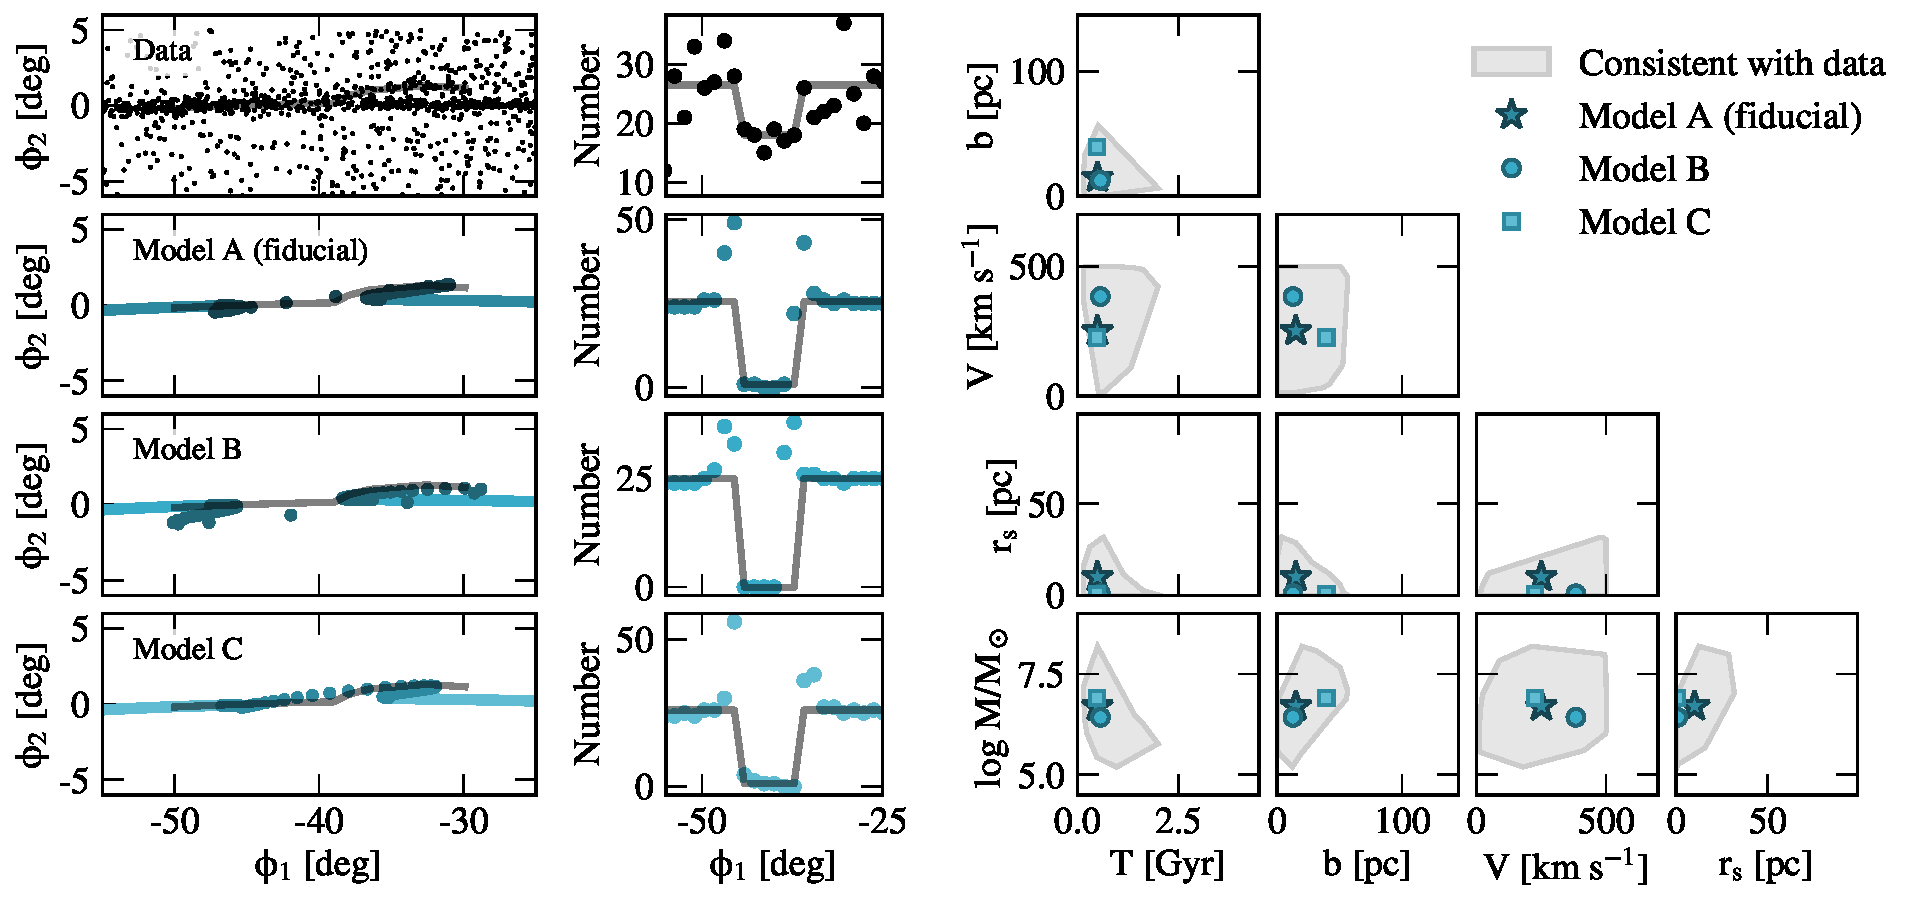
\includegraphics[width=\textwidth]{param_search.pdf}
\end{center}
\caption{(Left) Comparison of the observed GD-1 spur (left column) and gap (right column) in the top row to the modeled features in the bottom three rows. 
The gray line tracing the observed features was used for evaluating GD-1 models.
(Right) The parameter space of the allowed models is shaded gray, with the highlighted models falling inside this region.
The data prefer a recent, close encounter with a massive, dense object.
}
\label{fig:corner}
\end{figure*}

Decreasing the velocity of the perturber (which also increases the velocity kicks) produces larger loops and gaps, and this effect is nearly degenerate with an increase in perturber's mass at sufficiently large velocities.
However, at very low velocities, the whole loop morphology is changed (top panel in fourth column, Figure~\ref{fig:scalings}), likely because the encounter is no longer impulsive.
This means that the observed spur morphology cannot be explained by an object of an arbitrarily low mass moving slowly.
Likewise, decreasing the impact parameter has a unique signature too: the resulting loop is larger, but the gap size remains constant.

Different encounter parameters produce a unique impact on the GD-1 morphology, so we next search this space for parameter combinations allowed by the data.
Ideally, we would like to create a model of the stream and compare it to the data directly.
However, the adopted method for generating stream models is not sufficiently realistic for full forward-modeling.
Instead, we devised a set of expert criteria that allow us to compare whether a conceptual stream model represents the observed structure of GD-1.

First, we compare $\phi_2$ positions perpendicular to the stream of perturbed model stars to the position of observed stars in the spur, defined as a spline that goes through control points of the stream between $\phi_1=-50^\circ$ to $-39^\circ$, and control points on the spur between $\phi_1=-39^\circ$ to $-30^\circ$.
Positions of likely GD-1 members and this spline are shown in the top left of Figure~\ref{fig:corner} as black points and gray line, respectively.
Positions of stars in the fiducial model (A), and two other models (B and C) are shown in bottom rows, with darker colors marking stars with a significant change in energy due to the encounter (bracketed by the third percentile on the trailing end and the 92nd percentile of the energy difference on the leading end of the stream). 
Quantitatively, we define the spur chi-square:
\begin{equation}
\chi^2_{spur} = \frac{1}{N}\sum_{i=1}^{N} \left(\frac{\phi_{2,\,i} - \phi_{2,\,spline}(\phi_{1,\,i})}{\sigma_{spur}}\right)^2 
\end{equation}
for $N$ model stars with positions $(\phi_{1,\,i}, \phi_{2,\,i})$, and adopted width of the spur as $\sigma_{spur} = 0.2^\circ$.
To ensure that the model spur is long enough, we only consider models where at least one star has $\phi_1>-32^\circ$ and $\phi_2>0.8^\circ$.

Next, we compare the location and width of the observed and model gaps.
The observed gap profile is shown in the top panel of second column in Figure~\ref{fig:corner} (black points), and is well-represented by a top-hat profile centered on $\phi_{1,\,gap}=-40.5^\circ$ and $w_{gap}=8.5^\circ$ wide (gray line).
Gap profiles of models A through C have similar positions and widths, however, the density contrast between the gap and the spur is much larger (bottom rows).
As the predictions of our stream models regarding density are simplistic, we define the gap chi-square as:
\begin{equation}
\chi^2_{gap} = \frac{1}{N_{bin}}\sum_{i=1}^{N_{bin}} \left(\frac{N_{model}(\phi_{1,\,i}) - N_{top}(\phi_{1,\,i})}{\sigma_{gap,\,i}}\right)^2
\end{equation}
where $i$ denotes $N_{bin}=29$ bins between $-60^\circ<\phi_1<-20^\circ$.
$N_{model}(\phi_{1,\,i})$ is the number of model stars in bin $i$, and $\sigma_{gap,\,i}$ is the associated Poisson uncertainty.
$N_{top}(\phi_{1,\,i})\equiv N_{top}(n_{base}, n_{hat}, \phi_{1,\,gap}, w_{gap} | \phi_{1,\,i})$ is the number of stars expected in bin $i$ from a top-hat distribution with the position $\phi_{1,\,gap}$ and width $w_{gap}$ adopted from the observed profile, but with the base level, $n_{base}$, given by the median of the model profile outside of the gap ($-55^\circ<\phi_1<-45^\circ$ and $-35^\circ<\phi_1<-25^\circ$), and $n_{hat}$ is the median of the model profile in the gap ($-43^\circ<\phi_1<-37^\circ$).
We further require the density contrast $n_{hat} / n_{base}$ at least 0.5.

We combine the spur and gap contributions to the log likelihood as $\ln\mathcal{L} = -(\chi^2_{spur} + \chi^2_{gap})$.
Even though this likelihood is an approximation to the formal likelihood which would compare the positions of model stream stars to the observed ones, it is expected to favor models that reproduce well features (spur and gap) seen in the data (is this an instance of ABC?).
Therefore, we use an ensemble MCMC sampler \citep{Foreman-Mackey:2013} to find the allowed range in parameters of interest: perturber's mass, size, velocity, impact parameter and impact time, while marginalizing over the orientation angles and impact location.
We started 200 walkers and advanced them for 5000 steps, keeping the last 2000 steps for analysis.
In principle, the resulting chain provides posterior samples, but since this is a highly idealized search of the parameter space, we only provide plausible ranges of parameters, instead of showing their two-dimensional distributions.
Specifically, in each panel of the corner plot (Figure~\ref{fig:corner}, right) we show the two-dimensional convex hull of all models with likelihood above the 5th percentile (gray shaded regions).

High-likelihood models of the GD-1 stream have encounter parameters expected from the stream's sensitivity to different parameters (explored in Figure~\ref{fig:scalings}).
Recent encounters are favored, with most of the models having been perturbed within the last 1\,Gyr and none more than 2\,Gyr ago.
The perturbing object itself is massive ($5.5\lesssim\log M/\rm M_\odot\lesssim8$) and dense ($r_s\lesssim20\,\rm pc$).
A range of velocities are allowed, as the data dismiss only the slowest moving perturbers ($V\gtrsim50\,\rm km\,s^{-1}$).
The closest approach was extremely close to the stream, with the impact parameter smaller than $b\lesssim50\rm\,pc$.


\subsection{Predictions for the kinematic signatures of the encounter in GD-1}
\label{sec:kinematics}
Perturber properties presented in the previous section were constrained by the spatial distribution of the GD-1 debris alone.
We now explore kinematic signatures of the GD-1 encounter with such a perturber and discuss how to further constrain its properties with future kinematic observations.

\begin{figure}
\begin{center}
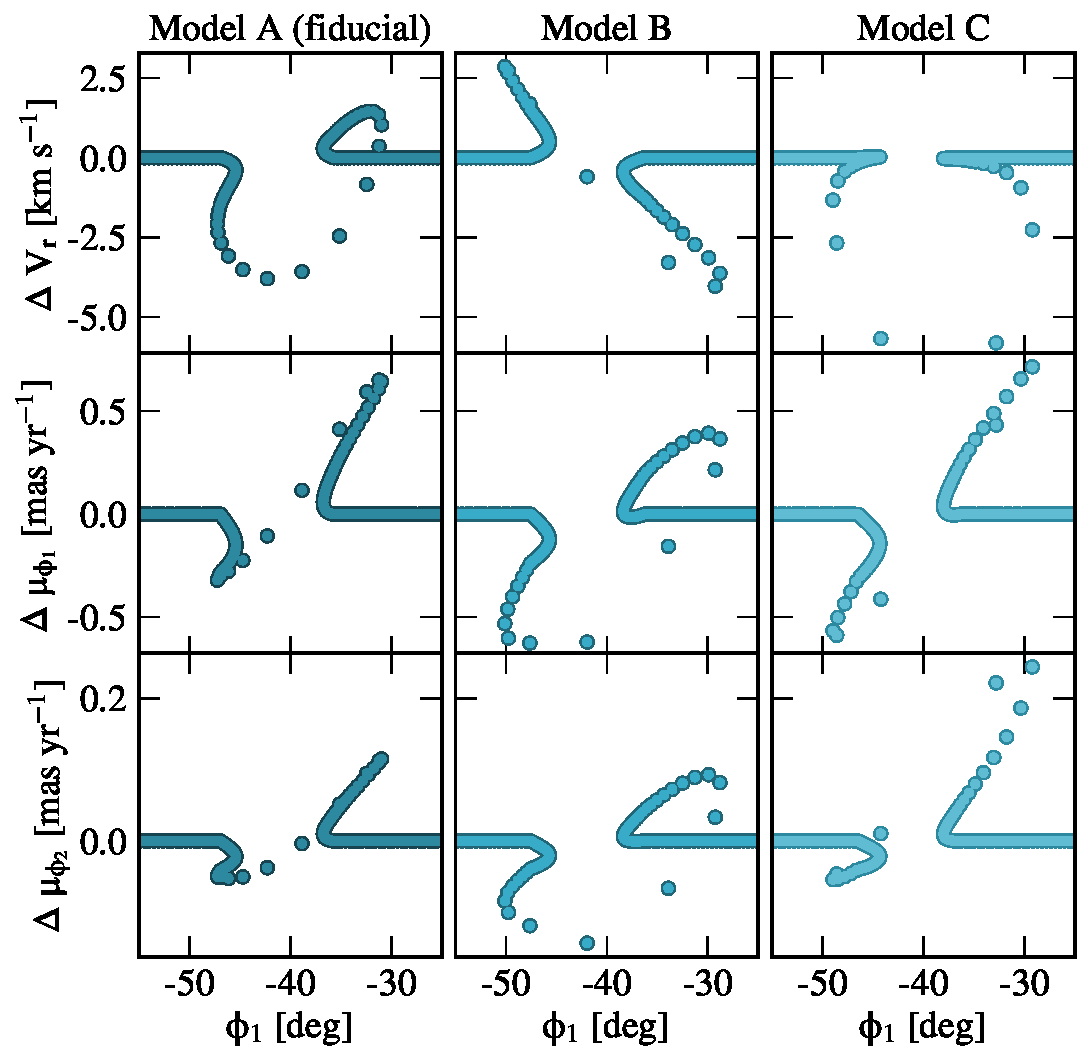
\includegraphics[width=\columnwidth]{kinematic_predictions.pdf}
\end{center}
\caption{Components of the relative velocity between the perturbed and unperturbed stream (with radial velocity on top, and proper motion along and perpendicular to the stream in the middle and bottom, respectively) for three different model streams (columns).
The direction of the offset in radial velocity depends on the encounter geometry and can constrain the perturber's orbit.
The direction of velocity offsets in proper motions is universal and can be used to falsify the encounter scenario.
}
\label{fig:predictions}
\end{figure}

In Figure~\ref{fig:corner} we introduced three models whose loops reproduce the observed spur and gap morphologies (left), and consequently, their encounter parameters are in the allowed region of the parameter space (right).
These particular models were selected to display the diversity in kinematic signatures of the loop allowed by the spatial data.
To account for the velocity gradients present along the stream, in Figure~\ref{fig:predictions} we show differences in velocity components between the perturbed and unperturbed stream for these three models.
Each column displays velocity signatures of a single model, with radial velocity differences in the top row, and the two proper motion components in GD-1 coordinates in the following rows.
In all of the models, there are kinematic offsets between the loop and the unperturbed stream.

Radial velocity signatures exhibit the largest diversity, most prominently manifested as the velocity difference between the spur and the unperturbed stream at $\phi_1\approx-30^\circ$.
Here, model A predicts the spur to move faster than the stream, in model B the stream moves faster than the spur, whereas there is no difference between the two in model C.
The other side of the loop has the opposite behavior, so models A and B predict bimodal radial velocity measurements in GD-1 stream at $-50^\circ\lesssim\phi_1\lesssim-45^\circ$.
The maximal offset in radial velocity is on the order of a few km\,s$^{-1}$, which is easily within reach of current spectroscopic facilities \citep[e.g.,][]{sg2007}.
The baseline radial velocity in the perturbed part of the stream is $\sim-100\,\rm km\,s^{-1}$ \citep{koposov2010}, allowing for confident selection of GD-1 members out of the field Milky Way population.
Models A, B, and C have rather similar parameters overall (Figure~\ref{fig:corner}, right), but the perturber's orbital plane is misaligned with that of GD-1 by $170^\circ$, $15^\circ$, and $50^\circ$, respectively.
Therefore, future follow-up observations will not only further constrain all impact parameters, but also provide first strong constraints on the encounter geometry.

Velocity offsets in proper motions have the same direction across all models (Figure~\ref{fig:predictions}, bottom two rows).
Focusing first on the $\phi_1$ direction, this behavior stems from the fact that there is a gap in the stream and that the stream moves in the negative $\phi_1$ direction (i.e., $\mu_{\phi_1}<0$).
As \citep{eb2015} showed, velocity kick along the stream (the $\phi_1$ direction) makes the affected stars on the leading side of the gap speed past the unperturbed stream.
And indeed, loop stars at $\phi_1\lesssim-45^\circ$ have proper motion $\mu_{\phi_1}$ more negative than the unperturbed stream at the same $\phi_1$.
The opposite behavior is expected, and seen, on the other side of the loop ($\phi_1\gtrsim-35^\circ$), where the affected stars lag behind the stream at less negative $\mu_{\phi_1}$.
Details of the loop proper motion offsets still depend on the perturber's parameters, but the direction of offsets along the stream is universal in the encounter scenario.

Because the spur is at positive $\phi_2$, its proper motion perpendicular to the stream (the $\phi_2$ direction) should be faster than that of the unperturbed stream stars.
As expected, $\Delta\mu_{\phi_2}>0$ for all of the models at $\phi_1\gtrsim-35^\circ$.
The other side of the loop is at most slightly offset from the main stream track, so $\Delta\mu_{\phi_2}$ is very small at $\phi_1\lesssim-45^\circ$.
Finally, the magnitude of kinematic offsets perpendicular to the stream ($\Delta\mu_{\phi_2}$) is universally smaller than along the stream ($\Delta\mu_{\phi_1}$).
This is also expected because the gap is much wider than the distance between the stream and the spur.

The encounter model makes falsifiable predictions for proper motion kinematics in the affected region of the GD-1 stream.
The predicted velocity offsets are small, but proper motions of diffuse, cold streams have been measured at this precision with the \hst\ \citep{sohn2016}, so future kinematic data will rule on the perturbative origin of GD-1 features.
Should the encounter scenario be confirmed, these new data will also make strong predictions on the orbit and present-day position of the pertuber.


\section{Discussion}
\label{sec:discussion}
We presented a model of the GD-1 stream which experienced a recent encounter with a massive, dense object.
This fly-by imparted significant velocity kicks to the closest stars both along the stream, which produced a gap in the stream, and perpendicular to the stream, which launched a spur of stars outside of the main stream.
The qualitative and quantitative agreement between the observed and modeled gap and spur suggest that these GD-1 structures are the first dynamical evidence for dark halo substructure.
Below we discuss how to ascertain this conclusion by suggesting improvements for future modeling of GD-1 (Section~\ref{sec:caveats}), reviewing possible origin scenarios of the observed features (Section~\ref{sec:origin}), and outlining strategies to distinguish these scenarios with additional observations (Section~\ref{sec:future}).

\subsection{Limitations of the current modeling setup}
\label{sec:caveats}
A number of simplifying assumptions were made to facilitate the initial modeling of complex features observed in the GD-1 stream.
While we expect these assumptions to still produce unbiased inference, there is a lot more information available in the present data than was employed so far.
We will need better models to fully explain these observations, so in this section we discuss areas for improvement in modeling of the GD-1 system.

Our fiducial model of GD-1 is built from test particles released by the disrupting progenitor directly from the Lagrange points, instead of particles dynamically ejected from the globular cluster progenitor itself.
Stream models generated under this assumption match the distribution of tidal debris (including the intrinsic density variations along the tidal tails) from direct N-body simulations while the progenitor persists \citep[e.g.,][]{kupper2012,fardal2015}.
However, the method is yet to be tested when the progenitor is completely disrupted, such as in the case of GD-1, and most of the known halo streams.
Last stages of tidal disruption can result in enhanced density variations \citep[e.g., for an exoplanet disruption, see][]{}, so to fully account for all the structures observed in GD-1 we will need a full N-body model of the stream.

Of course, the reason we decided against employing N-body models in this work is that they are computationally expensive, and prohibitively so for any kind of parameter space exploration.
This is why we further focused only on the perturbed region of GD-1 when inferring properties of its perturber, and assumed that all stars are on the same orbit.
Reassuringly, fiducial encounter parameters produce qualitatively similar features both in an idealized stream (Figure~\ref{fig:fiducial}) and in stars along a single orbit (Figure~\ref{fig:scalings}).
As discussed in Section~\ref{sec:perturber_properties}, this choice limited us to only matching positions of stream features, and to disregard density along the stream.
Since the density profile of the gap is also expected to contain information about the perturber \citep{eb2015b}, going forward we will need to have a proper generative model of the stream.

Furthermore, our treatment of the GD-1 perturber is also simplistic.
Although we explored perturbers of different masses and sizes, they all follow the \citet{hernquist1990} density profile.
This profile reduces to the point mass case in the limit of vanishing scale size, and is similar to the profile of dark matter halos \citep[NFW,][]{navarro1997} at small radii, although at larger radii it falls off more steeply as $r^{-4}$, compared to $r^{-3}$ for NFW halos.
While the inference of the perturber's scale radius should be robust to the details of its outer density profile, future work should explore whether any observables can be traced to the perturber's density structure, as it might hold additional clues to its origin.

In the absence of a realistic stream model, our inference of the GD-1 perturber was based on a set of high-level criteria instead of directly calculating the likelihood of the observed spatial distribution of tidal debris for a given set of model parameters \citep[e.g., likelihood developed in][]{bonaca2014}.
Spot-checking of the accepted models suggests we erred on the conservative side and accepted a wide range of models, some of which would likely be ruled out with the full likelihood.
For example, model B in Figure~\ref{fig:corner} has both sides of its loop appreciably offset from the stream track, instead of just the trailing side coinciding with the spur.
Because of that, with the current approach we only bound the allowed parameter space, and remain agnostic to the relative likelihood of models within the bounds.
To find preferred regions of the parameter space and recover the posterior density, future inference will need to employ a more realistic model of GD-1 and a proper likelihood.

And finally, our search of the parameter space has not been exhaustive, so different islands may still be allowed (for example, at a lower perturber mass or older encounter).
This is, of course, always true when sampling a parameter space \citep[appropriate mcmc reference][]{}.
However, ours is sufficiently low-dimensional that future studies employing the formal likelihood should be able to perform a brute-force sweep of the entire parameter volume and identify all classes of perturber properties that explain GD-1 features.

\subsection{Origin of GD-1 structures}
\label{sec:origin}
Many massive objects are known, or expected, to orbit the Galaxy, and if any should have encountered a cold stream, the perturbation would remain recorded in the stream's density profile.
So, the presence of perturbed features in GD-1 is not surprising, but their intricacy is.
In this section discuss what the observed structures suggest about their origin.

In this work we assumed that GD-1 was perturbed because of features in its density profile.
However, N-body simulations of disrupting globular clusters show that a certain level of structure in the resulting stream is intrinsic to the disruption process \citep[e.g.,][]{kupper2008,kupper2010}.
None of the present-day globular clusters would produce density variations as prominent as those observed in GD-1 \citep[see][]{pwb}, but if the GD-1 progenitor had a more complex internal structure than the known globular clusters, this might propagate to the morphology of its tidal tails and account for the observed features.
Non-trivial morphologies in stellar streams can also be produced by chaotic dispersal \citep{pw2016}.
For example, unexpectedly short lengths of the Ophiuchus and Palomar~5 streams have been attributed to chaos: in a chaotic potential featuring a rotating bar, large swaths of these streams can be dispersed to surface densities below our current detection threshold \citep{pw2016b,pearson2017}.
GD-1, on a retrograde orbit and with a larger pericenter than either of these streams, is deemed less susceptible to the chaotic influence of the rotating bar \citep{bb2018}.
Furthermore, the gap and spur features in GD-1 are much more localized than typical signatures of chaos in complex, time-dependent gravitational potentials, but there is still a lot of parameter space left to explore.

\begin{figure}
\begin{center}
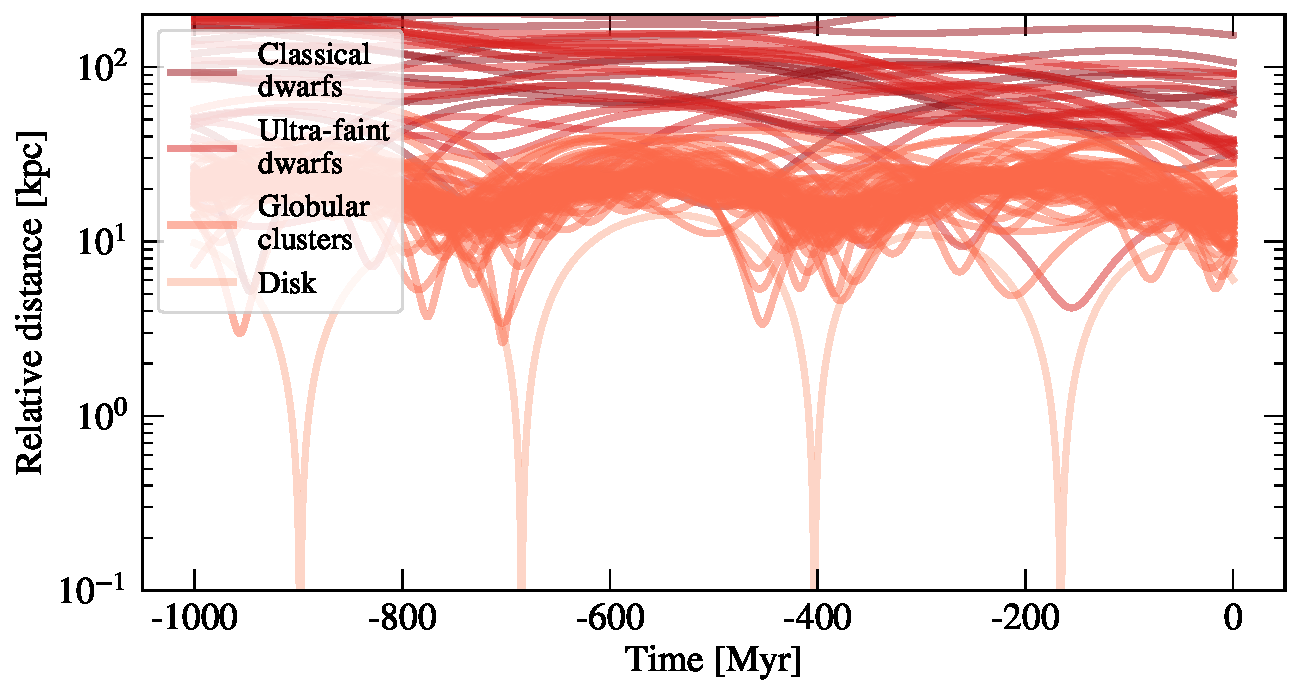
\includegraphics[width=\columnwidth]{satellite_distances.pdf}
\end{center}
\caption{Relative distance between the GD-1 gap and known objects in the Milky Way: classical dwarf galaxies (dark red), ultra-faint dwarfs (red), globular clusters (orange) and the stellar disk (light orange).
No known compact object approaches GD-1 close enough to produce the observed gap-and-spur features.
}
\label{fig:known_encounters}
\end{figure}

\begin{figure*}
\begin{center}
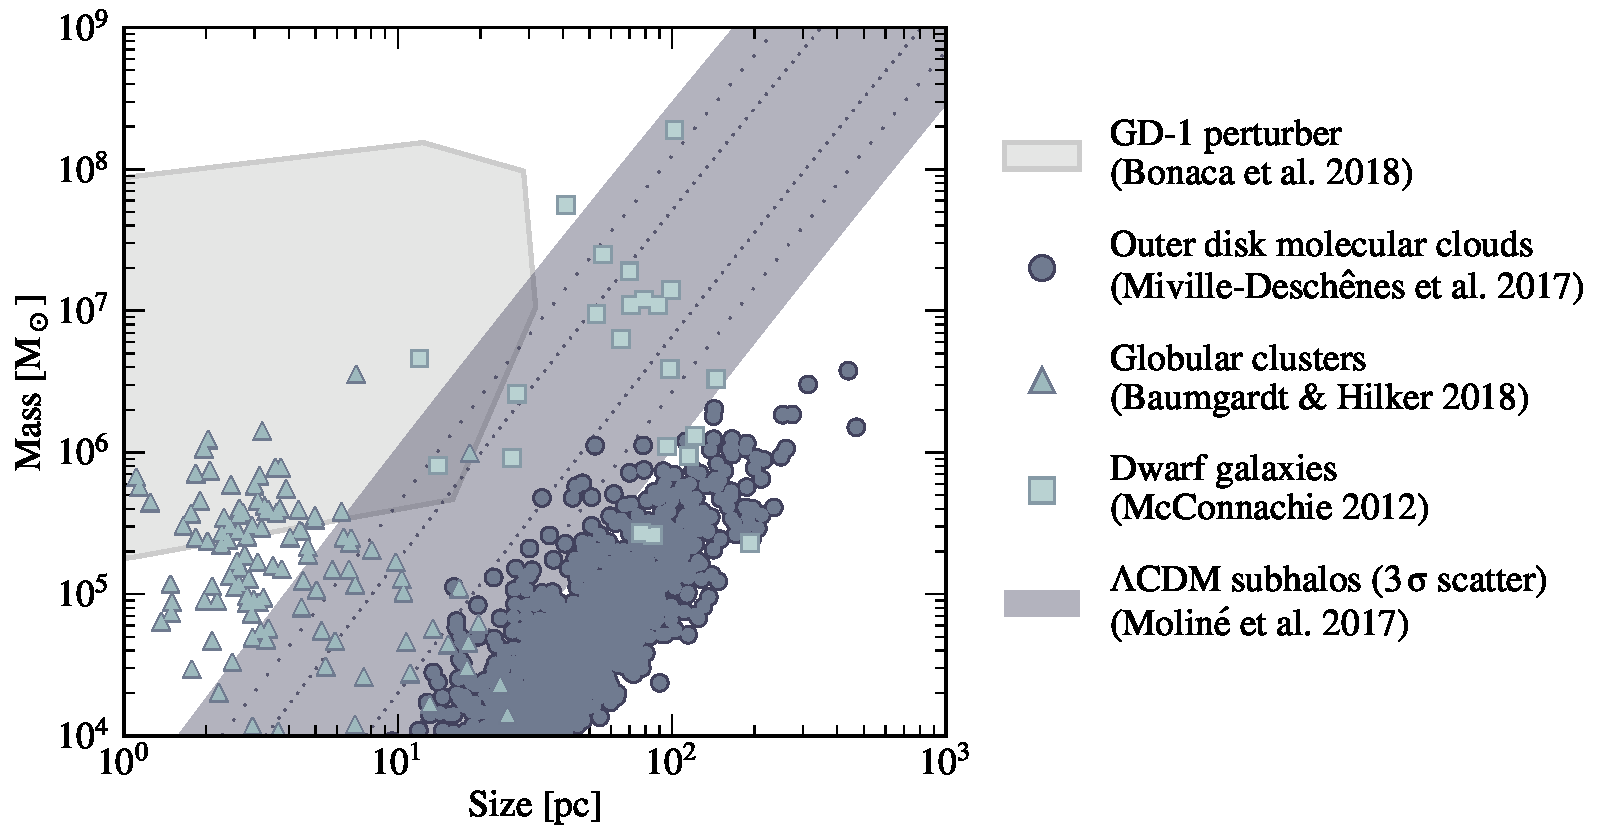
\includegraphics[width=0.9\textwidth]{mass_size.pdf}
\end{center}
\caption{Comparison of inferred mass and scale radius of the GD-1 perturber (following a Hernquist profile, light gray shaded region) to the known dwarf galaxies (squares), globular clusters (triangles), and molecular clouds in the outer disk (circles).
For dwarf galaxies and globular cluster we show the total mass and half-light radius, while for molecular clouds we show total mass and total size.
Molecular clouds are too diffuse to have caused features in the GD-1 stream.
The dark shaded region is showing masses and scale radii of dark matter halos (following an NFW profile) and the expected $3\,\sigma$ scatter.
GD-1 perturber is on the dense, or high-concentration, end of dark matter halos.
}
\label{fig:mass_size}
\end{figure*}

Getting back to the perturbation scenario: the Milky Way is surrounded by $\sim60$ dwarf galaxies \citep{mcconnachie2012} and $\sim160$ globular clusters \citep{harris2010}, most of which, same as GD-1, are residing in the halo.
Thanks to the \gaia\ mission, a significant fraction of these satellites are now fully located in the 6D phase space \citep{simon2018, gdr2_satellites}.
To test whether any of these objects could have perturbed GD-1, we integrated their orbits in a fiducial Milky Way potential \citep{pw2017} and show their relative distance from the GD-1 gap at $\phi_1=-40^\circ$ during the past billion years in Figure~\ref{fig:known_encounters}.
Lines are shaded according to the object's mass, with the classical dwarfs being the darkest, ultra-faints medium, and globular clusters lighter.
All of them have kept at least 1\,kpc away from GD-1.
Relative distances shown in Figure~\ref{fig:known_encounters} were calculated for fiducial present-day positions and velocities of satellites.
Since the associated measurement uncertainties can be substantial, we also sampled the error distribution and found that no satellite comes closer than x\,pc in any of the orbital samples.
The maximum impact parameter inferred for GD-1 perturbation is 57\,pc, thus disfavoring known satellites as perturbers of GD-1.

% We sample from the error distributions for each kinematic measurement of each satellite to assess whether any of the known Milky Way satellites could have come close to the location of the gap and spur location within the last 2\,Gyr.
% We generate 2048 samples of the present-day 6D phase-space positions for each satellite and integrate these orbits in our assumed 3-component Milky Way mass model (Price-Whelan et al. 2017, Bovy et al. 2015).
% We find that most satellites have no samples that come within 100 pc of the gap.
% Two globular clusters, NGC 6496 and IC 4499, come within 100 pc in 0.6\% and 0.2\% of their orbit samples, respectively.
% This suggests that none of the known Milky Way satellites with measured kinematics could be responsible for the observed density variations in GD-1, but we note that, for these two globular clusters, improved distance measurements would be needed to improve their orbits and definitely rule them out as perturbers.

As it orbits the Galaxy, GD-1 crosses the disk at timescales comparable to the inferred time of perturbation (the lightest line in Figure~\ref{fig:known_encounters} is the distance from the Galactic plane).
While strong disk shocking can facilitate disruption of a diffuse globular cluster \citep{dehnen2004}, GD-1 disk crossings are between 13\,kpc and 23\,kpc from the Galactic center, where the disk density is too low to significantly impact the stream, or produce sharp features such as the gap and the spur.
Still, giant molecular clouds (GMCs) that are orbiting in the disk plane can perturb cold stellar streams \citep{amorisco2016}.
To test whether GMCs are viable candidates for the GD-1 perturber, in Figure~\ref{fig:mass_size} we compare the inferred mass and size of the GD-1 perturber (gray shaded region) to known objects in the Milky Way, including molecular clouds.
Dwarf galaxies are shown as light squares \citep{mcconnachie2012}, globular clusters as medium triangles \citep{baumgardt2018}, and outer-disk molecular clouds (beyond 10\,kpc) as dark circles \citep{md2017}.
This comparison is rather conceptual as different classes of objects have different density profiles: for the GD-1 perturber we show the mass and scale radius assuming a Hernquist profile, for dwarf galaxies and globular clusters we show the total dynamical mass and half-light radius, and the total (high) mass and full size for molecular clouds.
Keeping these caveats in mind, the most massive globular clusters and the most compact dwarf galaxies have masses and sizes comparable to the preferred values of the GD-1 perturber, but GMCs are in general too diffuse.
To additionally test for extremely dense, yet undiscovered class of GMCs, we also created GD-1 models perturbed by a $10^7\,\rm M_\odot$ point mass moving on a circular disk orbit for the three most recent disk crossing times.
These configurations result in a spur that is below the stream at $\phi_2<0$, rather than above at $\phi_2>0$ as observed in GD-1, so we conclude that GMCs are unlikely to have perturbed GD-1.

Having ruled out known objects, we find that the most probable GD-1 perturber is a dark object in the Milky Way halo.
As luminous satellites can have approximately the required masses and sizes, a low luminosity unknown satellite might be the culprit.
To avoid detection, it would have to be fortuitously hiding in the disk plane, or moving very fast, as our best estimate is that the encounter was recent.
Near-future and upcoming surveys of the plane \citep{schlafly2018} and the halo \citep{lsst} should provide a complete census of objects in the Milky Way and find a perturber of low luminosity.

Alternatively, the GD-1 perturber could be completely dark.
A dense pertuber in the mass range $10^5-10^8\,\rm M_\odot$ is required, so we next discuss black holes -- the densest dark objects in the Universe.
Baryonic black holes of similar masses typically reside in centers of galaxies \citep[the mass of Milky Way's supermassive black hole, Sgr A$^\star$, is $\approx4\times10^6\,\rm M_\odot$][]{boehle2016}.
A population of non-baryonic, primordial black hole is hypothesized to have formed in the early universe \citep{carr1974}, and has sparked a renewed interest as a dark matter candidate following the LIGO detections \citep{bird2016}.
Several lines of inquiry have limited the contribution of massive ($\gtrsim10^3\,\rm M_\odot$) primordial black holes to the dark matter budget to less than $\lesssim0.1\,\%$ \citep[and references within]{carr2016}.
So if GD-1 encountered a primordial black hole, this would have been an extremely rare event, and we would not expect to see similar features in other streams upon a comparable amount of scrutiny.

On the other hand, $\Lambda$CDM cosmological simulations predict scores of dark matter subhalos orbiting Milky Way-like galaxies.
Even after accounting for the destruction of subhalos due to the stellar disk \citep{donghia2010,gk2017}, their density in the inner 20\,kpc is high enough that a stream on a GD-1-like orbit is expected to have encountered at least one $10^6-10^7\rm\, M_\odot$ subhalo within the last $\sim8$\,Gyr \citep{erkal2016}.
Of the two prominent gaps in GD-1, our fiducial model ascribes one to the site of the progenitor's disruption, and one to the encounter with a perturber.
Thus, a dark matter subhalo is a plausible GD-1 perturber in terms of encounter rates expected in the $\Lambda$CDM universe.

The high inferred density of the GD-1 perturber makes it more resilient to disruption in the tidal field of the inner galaxy, but preferred values are on the high end of dark matter halo concentrations.
The dark shaded band in Figure~\ref{fig:mass_size} shows the $3\,\sigma$ scatter in masses ($M_{200,c}$) and sizes (NFW scale radii, $r_s$) of isolated dark matter halos \citep{diemer2018}.
There is minimal overlap between dark matter halo properties and the GD-1 perturber under the assumption of constant scatter, but the fraction of high-concentration halos increases at low masses \citep{diemer2015}, and has not been quantified below $<10^{10}\,\rm M_\odot$.
Furthermore, studies of subhalos at higher masses show that subhalos in dense environments are more concentrated than field halos of the same mass \citep[e.g.,][]{avilareese2005}.
Although more theoretical work is needed to fully establish properties of low-mass subhalos in the inner Galaxy, a dark matter subhalo is a plausible candidate for the GD-1 perturber based on structural parameters as well.

% Current $\Lambda$CDM simulations can easily be extended to the relevant spatial ($r\lesssim30\,kpc$) and mass scales ($10^5<M/\rm M_\odot<10^8$) to establish 
% further motivated by the changes in the density profile of subhalos upon accretion \citep{dicintio2013}.
% - and as details of the profile would matter here, further work required in modeling, but most likely, we will need additional data to fully constrain it
% Cosmological significance of a low-mass dark matter subhalo detection implores follow-up of these GD-1 features, and we provide specific strategies in the next section.

% Regardless of their origin, features seen in GD-1 are a result of an interesting event.
% The stream either originates from an unusual progenitor, has been shaped by a curious dynamical effect, or encountered an unknown perturber.
% The perturbation scenario presented in this work has a unique kinematic signature, so we next discuss how to direct future observations and definitively ascertain the origin of GD-1 features.

% - give some typical dm substructure numbers for the whole galaxy and for this radius range in the nearby halo.
% - also something about the mass-size relationship for these dm structures.
% - conclusion: dm substructure is the most plausible of the options.
% - interesting point: The predictions about \lcdm\ substructure in the inner halo are controversial right now because of simulation differences. If this matters, this point should enter the abstract and modify the naturalness of the conclusion.

\subsection{Future prospects}
\label{sec:future}
- we think perturbation by a dm subhalo is the most likely
- below we outline a set of observational and theoretical steps to be taken that can consolidate this picture
- we close with an outlook for studies of the dynamical halo

- confirmation:
- delta rv, mu
- not only confirm, but also get the orbit

- characterization:
- microlensing signatures in the searchbox
- better theoretical predictions on the density profile expected of dm subhalos
- high-velocity ejections?

- non-dynamical observables:

In summary, we suggest the following to definitively ascertain the origin of features in the GD-1 stream:
\begin{enumerate}
 \item measure precise relative radial velocity between the spur and the stream
 \item measure precise relative proper motions between the spur and the stream
 \item find the orbit of the perturber and search for microlensing signals at its present-day location
 \item characterize simulated dark matter subhalos at low masses in the inner halo
 \item search for emission from the perturber
\end{enumerate}

GD-1 stream is a beautiful display of information encoded in cold stellar streams, perturbation in a lot of detail
This breakthrough is entirely due to the data provided by the \gaia\ mission, and this study of the GD-1 gap-and-spur feature is only a pathfinder.
There is another similar feature in GD-1 (the blob), as well as more than 40 cold streams orbiting between 5 and 40\,kpc, that can be analogously analyzed.
With enough events, we may be able to measure the mass function of objects in the Milky Way halo.
And if the network of streams is sufficiently dense, we may even imagine tracking gravitational disturbances from a single object dynamically through time.


% The stream perturbation models presented above show that the GD-1 stream spur and neighboring gap could plausibly be formed through a gravitational interaction between the stream and a dark, compact, massive perturber.
% By assuming this scenario for the spur and gap formation, we have compared perturbed stream models to the observed gap location and width and spur location and length, and have determined regions of encounter parameter-space that reproduce the observed morphology of the GD-1 stream.
% In this context, we have shown that the perturber would have to be a massive but compact, fast-moving object in the halo of the Milky Way.
% 
% \lcdm\ predicts that subhalos with masses between $10^6~\msun < M < 10^8~\msun$ should be abundant...
% [observed dwarfs around the Milky Way are proof of $10^7$--$10^8~\msun$]
% However, [scale radii $\sim 10$ times larger, less dense]
% 
% - compare properties to expectation from dark matter, discuss black hole possibility (but also cool!)
% 
% - Return to discussion of low-mass subhalos in simulations: baryonic sims predict far fewer subhalos, but dense ones survive? Also crazy-time: LMC replenishing subhalo population
% 
% \subsection{Alternative explanations of the spur and gap}
% % This doesn't have to remain a subsection - just putting it here for organizing
% % my thoughts!
% - When discussing alternatives: Why are they less plausible? How could we rule them out in the future, or are they ruled out now?
% 
% - SMBH: more massive than MW SMBH - where is progenitor? how did it grow?
% - GMC in disk: wrong relative velocity as GD-1 crosses midplane
% - Internal kinematics of progenitor: fine-tuned to get gap
% - Feathering from stream formation: oriented wrong way w.r.t. GD-1 orbit
% - Stream-fanning: need strong chaos for stream bifurcation. far from bar, halo likely close to spherical within orbit of GD-1
% - Luminous dwarf or globular cluster: either (1) known systems have wrong kinematic measurements, (2) unseen / unknown system, or (3) Milky Way mass distribution very different than expected. Could show difference of orbit over last 500 Myr in different potential models
% 
% 
% \section{Conclusions}
% 
% - This is huge!
% - Optimistic future of a huge network of cold streams---what might be possible?


\acknowledgements
It is a pleasure to thank Vasily Belokurov, Warren Brown, Benedikt Diemer, Elena D'Onghia, Adrienne Erickcek, Douglas Finkbeiner, Lars Hernquist, Kathryn Johnston, Sergey Koposov, Doug Lin, Barry McKernan, Erica Nelson, Sarah Pearson, Hans-Walter Rix, and Josh Speagle for valuable discussions and input.

This project was developed in part at the 2018 \acronym{NYC} \Gaia\ \acronym{DR2} Workshop at the Center for Computational Astrophysics of the Flatiron Institute in New York City in 2018 April.

This work was performed in part at Aspen Center for Physics, which is supported by National Science Foundation grant PHY-1607611.

This work has made use of data from the European Space Agency (\acronym{ESA}) mission \Gaia\ (\url{https://www.cosmos.esa.int/gaia}), processed by the \Gaia\ Data Processing and Analysis Consortium (\acronym{DPAC}, \url{https://www.cosmos.esa.int/web/gaia/dpac/consortium}). Funding for the \acronym{DPAC} has been provided by national institutions, in particular the institutions participating in the \Gaia\ Multilateral Agreement.


\software{
\package{Astropy} \citep{astropy:2013, astropy:2018},
\package{colossus} \citep{diemer2018},
\package{gala} \citep{pw2017},
\package{emcee} \citep{Foreman-Mackey:2013},
\package{IPython} \citep{Perez:2007},
\package{matplotlib} \citep{Hunter:2007},
\package{numpy} \citep{Van-der-Walt:2011},
\package{scipy} \citep{scipy}
}

\bibliographystyle{aasjournal}
\bibliography{spur}

\end{document}
